\begin{figure}[h]\centering
    \begin{subfigure}{.4\textwidth}
            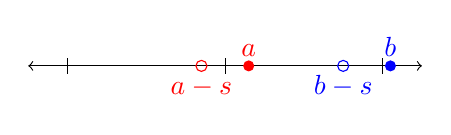
\begin{tikzpicture}
            \draw[<->] (-.5,0) -- (4.5,0);
            \foreach \x in {0,2,4}{
                \draw[] (\x,.1) -- (\x,-.1);
            }
            \fill[red] (2.3,0) node[above] {\(a\)} circle (2pt);
            \fill[blue] (4.1,0) node[above] {\(b\)} circle (2pt);
            \draw[red] (2.3-.6,0) node[below] {\(\phantom{b}a-s\phantom{b}\)} circle (2pt);
            \draw[blue] (4.1-.6,0) node[below] {\(b-s\)} circle (2pt);
            \end{tikzpicture}
        \caption{\( |a-b| \geq 1 \)}
        \label{c1}
    \end{subfigure}
    \begin{subfigure}{.4\textwidth}
            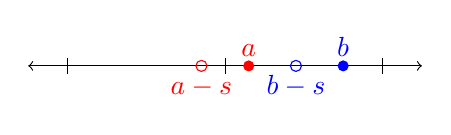
\begin{tikzpicture}
            \draw[<->] (-.5,0) -- (4.5,0);
            \foreach \x in {0,2,4}{
                \draw[] (\x,.1) -- (\x,-.1);
            }
            \fill[red] (2.3,0) node[above] {\(a\)} circle (2pt);
            \fill[blue] (3.5,0) node[above] {\(b\)} circle (2pt);
            \draw[red] (2.3-.6,0) node[below] {\(\phantom{b}a-s\phantom{b}\)} circle (2pt);
            \draw[blue] (3.5-.6,0) node[below] {\(b-s\)} circle (2pt);
            \end{tikzpicture}
        \caption{\(|a-b|<1, ~ s\in (a-\lfloor a \rfloor , b - \lfloor b \rfloor ) \)} 
        \label{c2}
    \end{subfigure}
    \begin{subfigure}{.4\textwidth}
            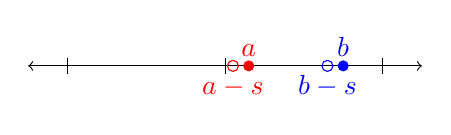
\begin{tikzpicture}
            \draw[<->] (-.5,0) -- (4.5,0);
            \foreach \x in {0,2,4}{
                \draw[] (\x,.1) -- (\x,-.1);
            }
            \fill[red] (2.3,0) node[above] {\(a\)} circle (2pt);
            \fill[blue] (3.5,0) node[above] {\(b\)} circle (2pt);
            \draw[red] (2.3-.2,0) node[below] {\(\phantom{b}a-s\phantom{b}\)} circle (2pt);
            \draw[blue] (3.5-.2,0) node[below] {\(b-s\)} circle (2pt);
            \end{tikzpicture}
        \caption{\(|a-b|<1, ~ s\in [0, a-\lfloor a \rfloor]\)} 
        \label{c3}
    \end{subfigure}
    \begin{subfigure}{.4\textwidth}
            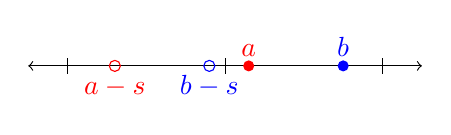
\begin{tikzpicture}
            \draw[<->] (-.5,0) -- (4.5,0);
            \foreach \x in {0,2,4}{
                \draw[] (\x,.1) -- (\x,-.1);
            }
            \fill[red] (2.3,0) node[above] {\(a\)} circle (2pt);
            \fill[blue] (3.5,0) node[above] {\(b\)} circle (2pt);
            \draw[red] (2.3-1.7,0) node[below] {\(\phantom{b}a-s\phantom{b}\)} circle (2pt);
            \draw[blue] (3.5-1.7,0) node[below] {\(b-s\)} circle (2pt);
            \end{tikzpicture}
            \caption{\(|a-b|<1, ~ s\in [b - \lfloor b \rfloor, 1) \)} 
        \label{c4}
    \end{subfigure}
    \caption{}
\end{figure}
        

